\documentclass[12pt,a4paper]{article}
\usepackage{ctex}
\usepackage{amsmath,amscd,amsbsy,amssymb,latexsym,url,bm,amsthm}
\usepackage{epsfig,graphicx,subfigure}
\usepackage{enumitem,balance}
\usepackage{wrapfig}
\usepackage{mathrsfs,euscript}
\usepackage[usenames]{xcolor}
\usepackage{hyperref}
\usepackage[vlined,ruled,linesnumbered]{algorithm2e}
\usepackage{array}
\hypersetup{colorlinks=true,linkcolor=black}

\newtheorem{theorem}{Theorem}
\newtheorem{lemma}[theorem]{Lemma}
\newtheorem{proposition}[theorem]{Proposition}
\newtheorem{corollary}[theorem]{Corollary}
\newtheorem{exercise}{Exercise}
\newtheorem*{solution}{Solution}
\newtheorem{definition}{Definition}
\theoremstyle{definition}

\renewcommand{\thefootnote}{\fnsymbol{footnote}}

\newcommand{\postscript}[2]
 {\setlength{\epsfxsize}{#2\hsize}
  \centerline{\epsfbox{#1}}}

\renewcommand{\baselinestretch}{1.0}

\setlength{\oddsidemargin}{-0.365in}
\setlength{\evensidemargin}{-0.365in}
\setlength{\topmargin}{-0.3in}
\setlength{\headheight}{0in}
\setlength{\headsep}{0in}
\setlength{\textheight}{10.1in}
\setlength{\textwidth}{7in}
\makeatletter \renewenvironment{proof}[1][Proof] {\par\pushQED{\qed}\normalfont\topsep6\p@\@plus6\p@\relax\trivlist\item[\hskip\labelsep\bfseries#1\@addpunct{.}]\ignorespaces}{\popQED\endtrivlist\@endpefalse} \makeatother
\makeatletter
\renewenvironment{solution}[1][Solution] {\par\pushQED{\qed}\normalfont\topsep6\p@\@plus6\p@\relax\trivlist\item[\hskip\labelsep\bfseries#1\@addpunct{.}]\ignorespaces}{\popQED\endtrivlist\@endpefalse} \makeatother

\begin{document}
\noindent

%========================================================================
\noindent\framebox[\linewidth]{\shortstack[c]{
\Large{\textbf{Lab07-Amortized Analysis}}\vspace{1mm}\\
CS214-Algorithm and Complexity, Xiaofeng Gao \& Lei Wang, Spring 2021.}}
\begin{center}
\footnotesize{\color{red}$*$ If there is any problem, please contact TA Yihao Xie. }

\footnotesize{\color{blue}$*$ Name:RenyangGuan  \quad Student ID:519021911058 \quad Email: guanrenyang@sjtu.edu.cn}
\end{center}
\begin{enumerate}
	\item Suppose we perform a sequence of n operations on a data structure in which the $i$ th 		operation costs $i$ if $i$ is an exact power of 2, and 1 otherwise. Use an accounting method to determine the amortized cost per operation.
    \begin{solution}
    Define the actual cost of the operation $i$ is $C_i$ and we have
    \begin{equation}
        C_i=
        \begin{cases}
        i & i\ is \ the \ power \ of \ 2\\
        1 & otherwise
        \end{cases}
    \end{equation}
    Assuming $n=2^k$, then the actual total cost is 
	\begin{equation}
	        \sum_{i=1}^n C_i=1+2+(1)+4+(1+1+1)+8+\cdots +(2^{k-1}-1)+2^k+\cdots
	\end{equation}
	We could think $2^{k-1} -1$ $1$s and one $2^k$ of an unit. If $i$ is not a power of $2$, the $\hat{C_i}$ acts as a prepaid credit. The credit will be used later for the nearest operation with $i$ equaling to a power of $2$.
	Based on the consideration, we could generate the amotsized cost as follows:
	
	\begin{table}[htbp]
	    \centering
	    \begin{tabular}{c|c|c}
	           \hline
	          Operation & Read Cost $C_i$ & Amortized Cost $\hat{C_i}$ \\
	         \hline
	         $i$ is a power of $2$ & i & $0$ \\
	          $i$ is not a power of $2$ &1 & $4$ \\
	       \hline
	    \end{tabular}
	\end{table}
    Because 
    \begin{align}
        \begin{split}
            \sum_{i=1}^n C_i &=1+2+4+8+\cdots +2^k+\\ &(2^1-1)+(2^2-1)+\cdots + (2^{k-1}-1)+t\\
            &=2^{k+1}-1+2(2^{k-1}-1)+k-1\\
            & =3\times 2^k+k-3\\
            &< 3n+\log n -3\\
            &< 4n
        \end{split}
        \begin{split}
            \sum_{i=1}^n \hat{C_i}
            &=4(2^-1+2^2-1+\cdots +2^k-1)\\
            &=4\times (2^k-3+k)\\
            &=4\times (n+\log n -3)\\
            &>4n\\
            &>\sum_{i=1}^n C_i
        \end{split}
    \end{align}
    The amortized cost analysis above is true and the amortized cost of each operation is $O(1)$.
    \end{solution}
	\item Consider an ordinary \textbf{binary min-heap} data structure with $n$ elements supporting
the instructions \textsc{Insert} and \textsc{Extract-Min} in $O(\log n)$ worst-case time. Give a
potential function $\Phi$ such that the amortized cost of \textsc{Insert} is $O(\log n)$ and the
amortized cost of \textsc{Extract-Min} is $O(1)$, and show that it works.
	\begin{solution}
	~\\
	\textbf{\textit{Basic consideration:}} An element must be inserted into the binary min-heap before being extracted. As a result, the \textsc{Insertion} operation prepays the \textit{credit}, which will be used by \textsc{EXTRACT-MIN}.
	\\
	\textbf{\textit{Potential function}}
    \begin{align}
        \Phi(n)=n\log n 
    \end{align}
    where $n$ is the number of elements in the heap.
    \\
    \\
    \textbf{\textit{Proof:}}
    \\
    \textbf{Proof for correctness:}
    Since the worst-case cost of both \textsc{INSERT} and \textsc{EXTRACT-MIN} is $O(\log n)$, the total amortized cost is 
    \begin{align*}
        \sum_{i=1}^n \hat{C_i}
        &= \sum_{i=1}^n C_i+\Phi (n)-\Phi (1)\\
        &= n\log n+n\log n\\
        &= 2n\log n\\
        &> \sum_{i=1}^n C_i
    \end{align*}
    \textbf{Proof for the question requirement:}
    \\
    \textit{Case 1:} the $n^{th}$ operation is \textsc{INSERT:}
    \begin{align}
        \hat{C_n}
        &= C_n+\Phi(S_{n})-\Phi(S_{n-1})\\
        &= \log n+n\log n- (n-1)\log (n-1)\\
        &= \log n+n\log \frac{n}{n-1}+\log (n-1)\\
        &= \Theta(\log n)+ \Theta(1) + \Theta(\log n)\\
        &= \Theta(\log n)
    \end{align}
    \\
    \textit{Case 2:} the $n^{th}$ operation is \textsc{EXTRACT-MIN:}
    \begin{align}
        \hat{C_n}
        &= C_n+\Phi(S_n)-\Phi(S_{n-1})\\
        &= \log n+n\log n- (n+1)\log (n+1)\\
        &= (n+1)\log \frac{n}{n+1}\\
        &= \Theta(1)
    \end{align}
    Since $C_n$ is the worst case time complexity of the $n^{th}$ operation and $\hat{C_i}$ gives an upper bound of $C_i$, the time complexity of \textsc{INSERT} is $O(\log n)$ and that of \textsc{EXTRACT-MIN} is $O(1)$.
    
    \end{solution}	
	
	\item Assume we have a set of arrays $A_0, A_1, A_2,\cdots$, where the $i^{th}$ array $A_i$ has a length of $2^i$. Whenever an element is inserted into the arrays, we always intend to insert it into $A_0$. If $A_0$ is full then we pop the element in $A_0$ off and insert it with the new element into $A_{1}$. (Thus, if $A_{i}$ is already full, we recursively pop all its members off and insert them with the elements popped from $A_0,...,A_{i-1}$ and the new element into $A_{i+1}$ until we find an empty array to store the elements.) An illustrative example is shown in Figure \ref{Fig-MultiArray}. Inserting or popping an element take $O(1)$ time.

	\begin{figure}[!htbp]
	\centering
	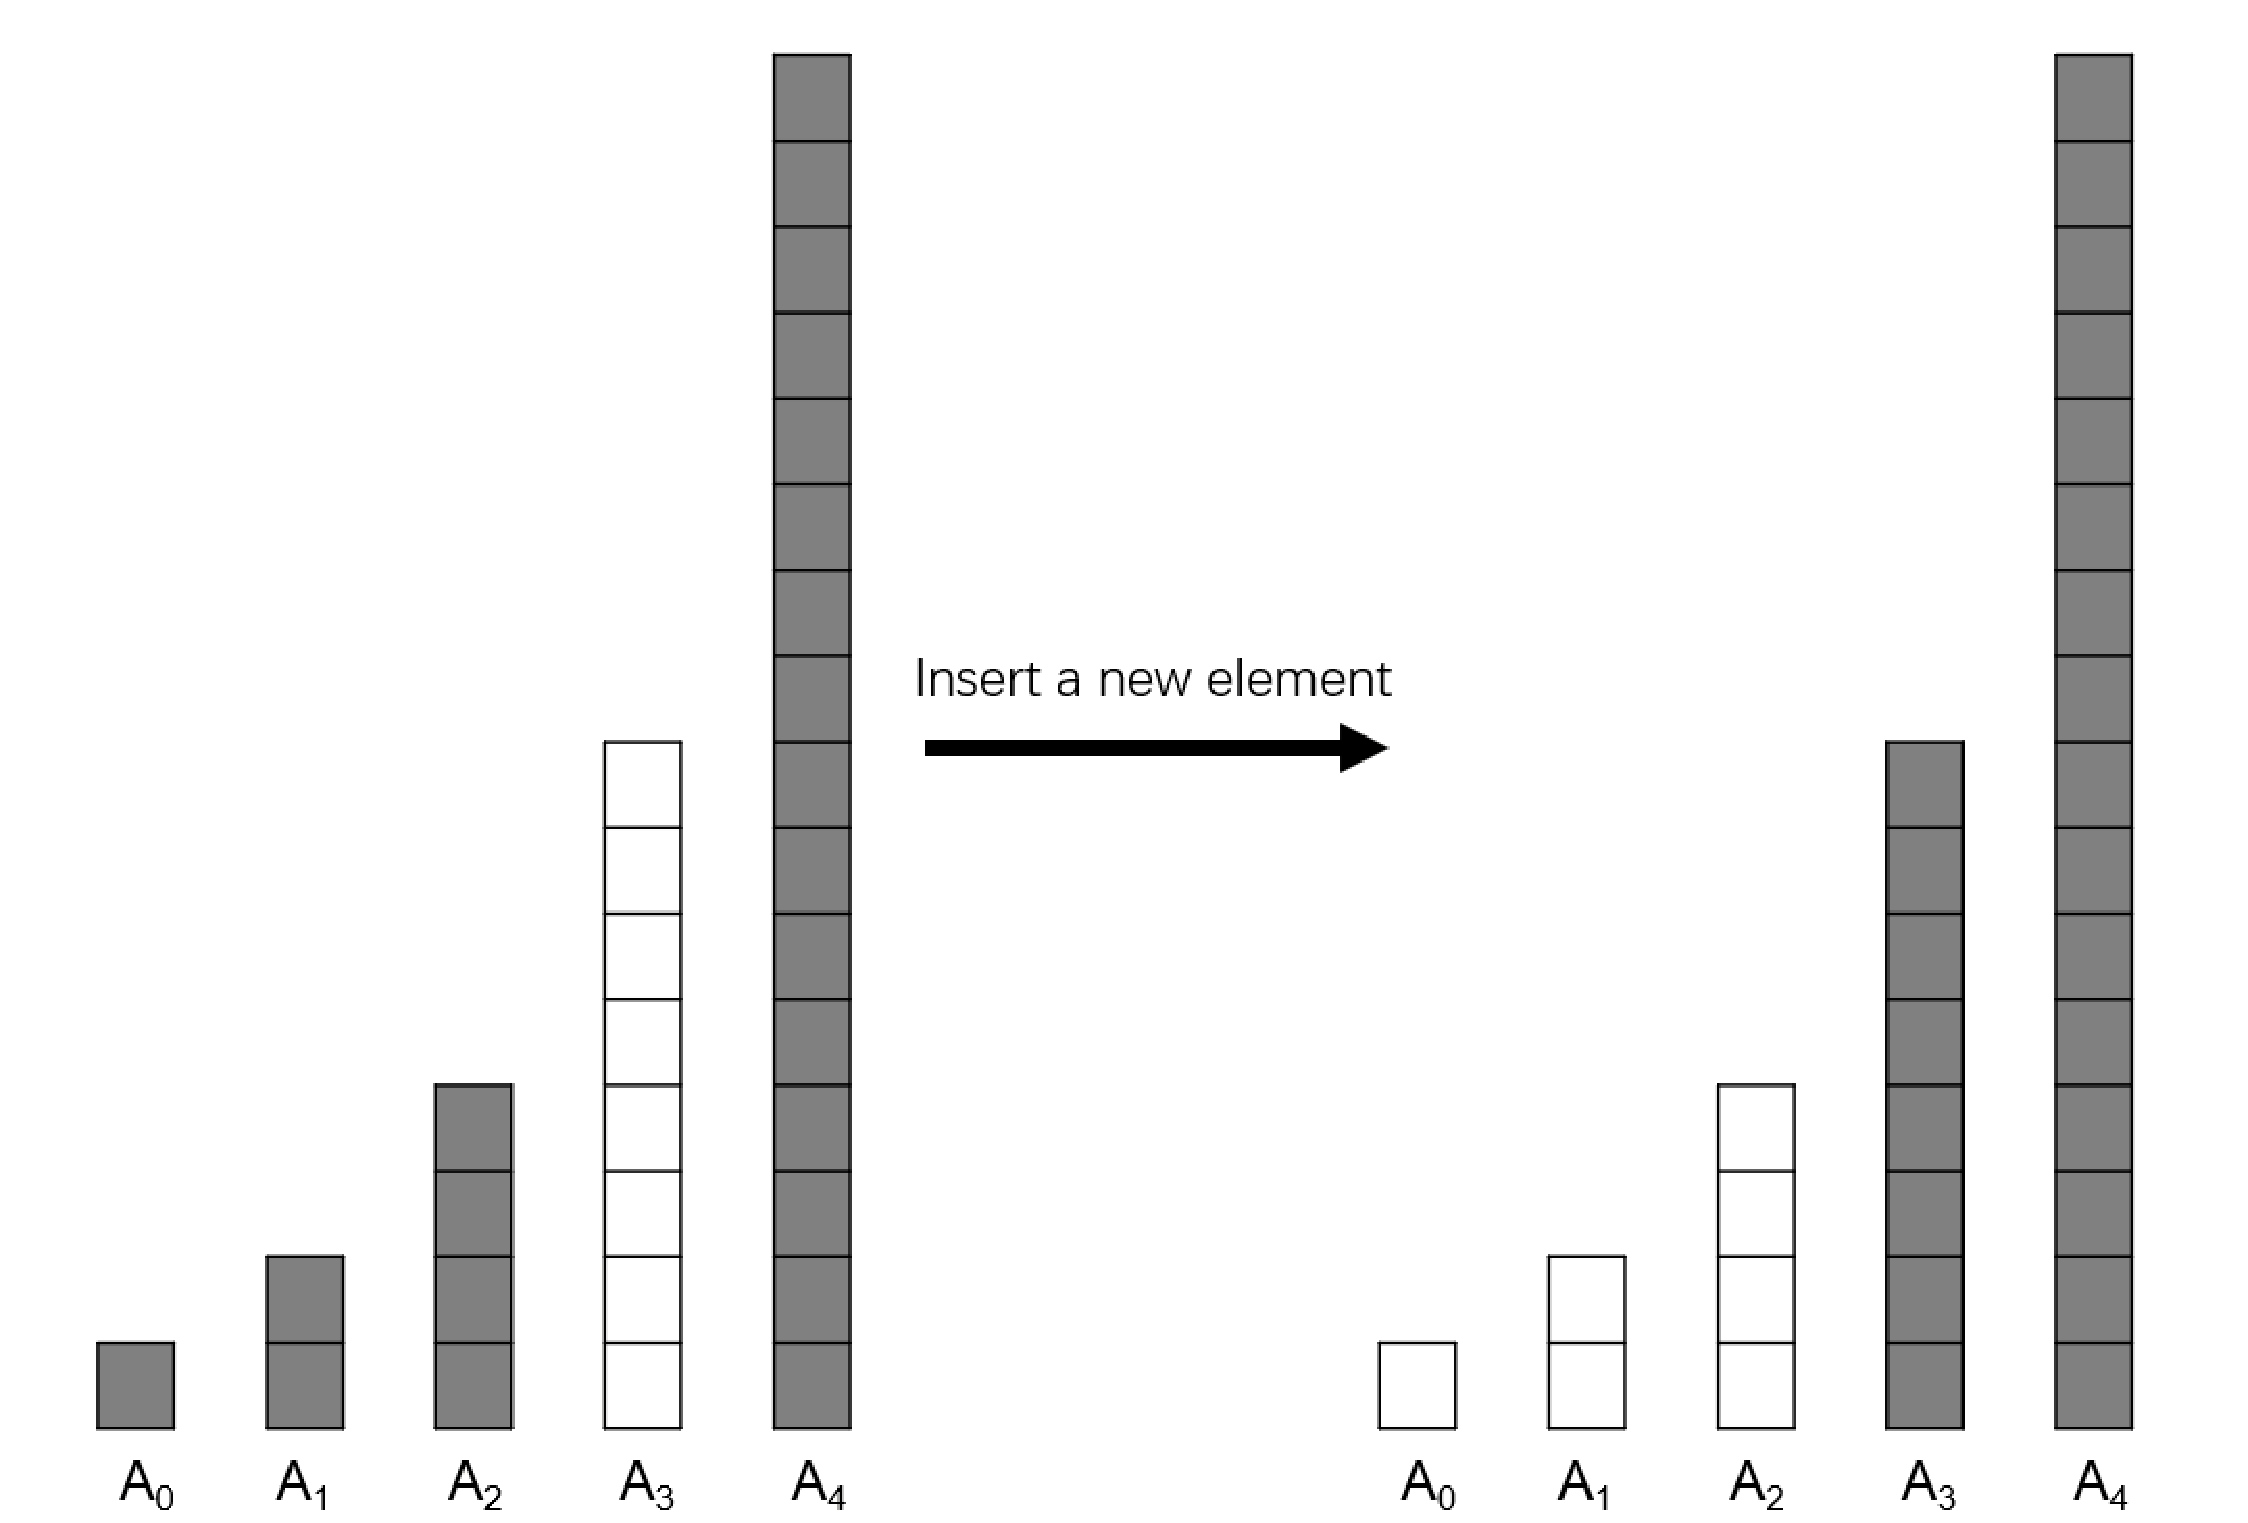
\includegraphics[width=0.5\textwidth]{Fig-MultiArray.pdf}
	\caption{An example of making room for one new element in the set of arrays.}
	\label{Fig-MultiArray}
	\end{figure}

    \begin{enumerate}
        \item In the worst case, how long does it take to add a new element into the set of arrays containing $n$ elements?
        \item Prove that the amortized cost of adding an element is $O(\log n)$ by \emph{Aggregation Analysis}.
        \item If each array $A_i$ is required to be sorted but elements in different arrays have no relationship with each other, how long does it take in the worst case to search an element in the arrays containing $n$ elements? 
\item What is the amortized cost of adding an element in the case of (c) if the comparison between two elements also takes $O(1)$ time?
    \begin{solution}
    ~\\
    \begin{enumerate}
        \item [(a)] For the sake of connevence, aussume $n=2^k-1$. The worst case occurs when n occupies $[A_0,A_1,\cdots,A_{k-1}]$. All of the n elements have to be popped out to insert the $n+1$ elements. As a result, it takes $O(n)$ to add a new element in the worst case.

        \begin{figure}[htbp]
        	\centering
        	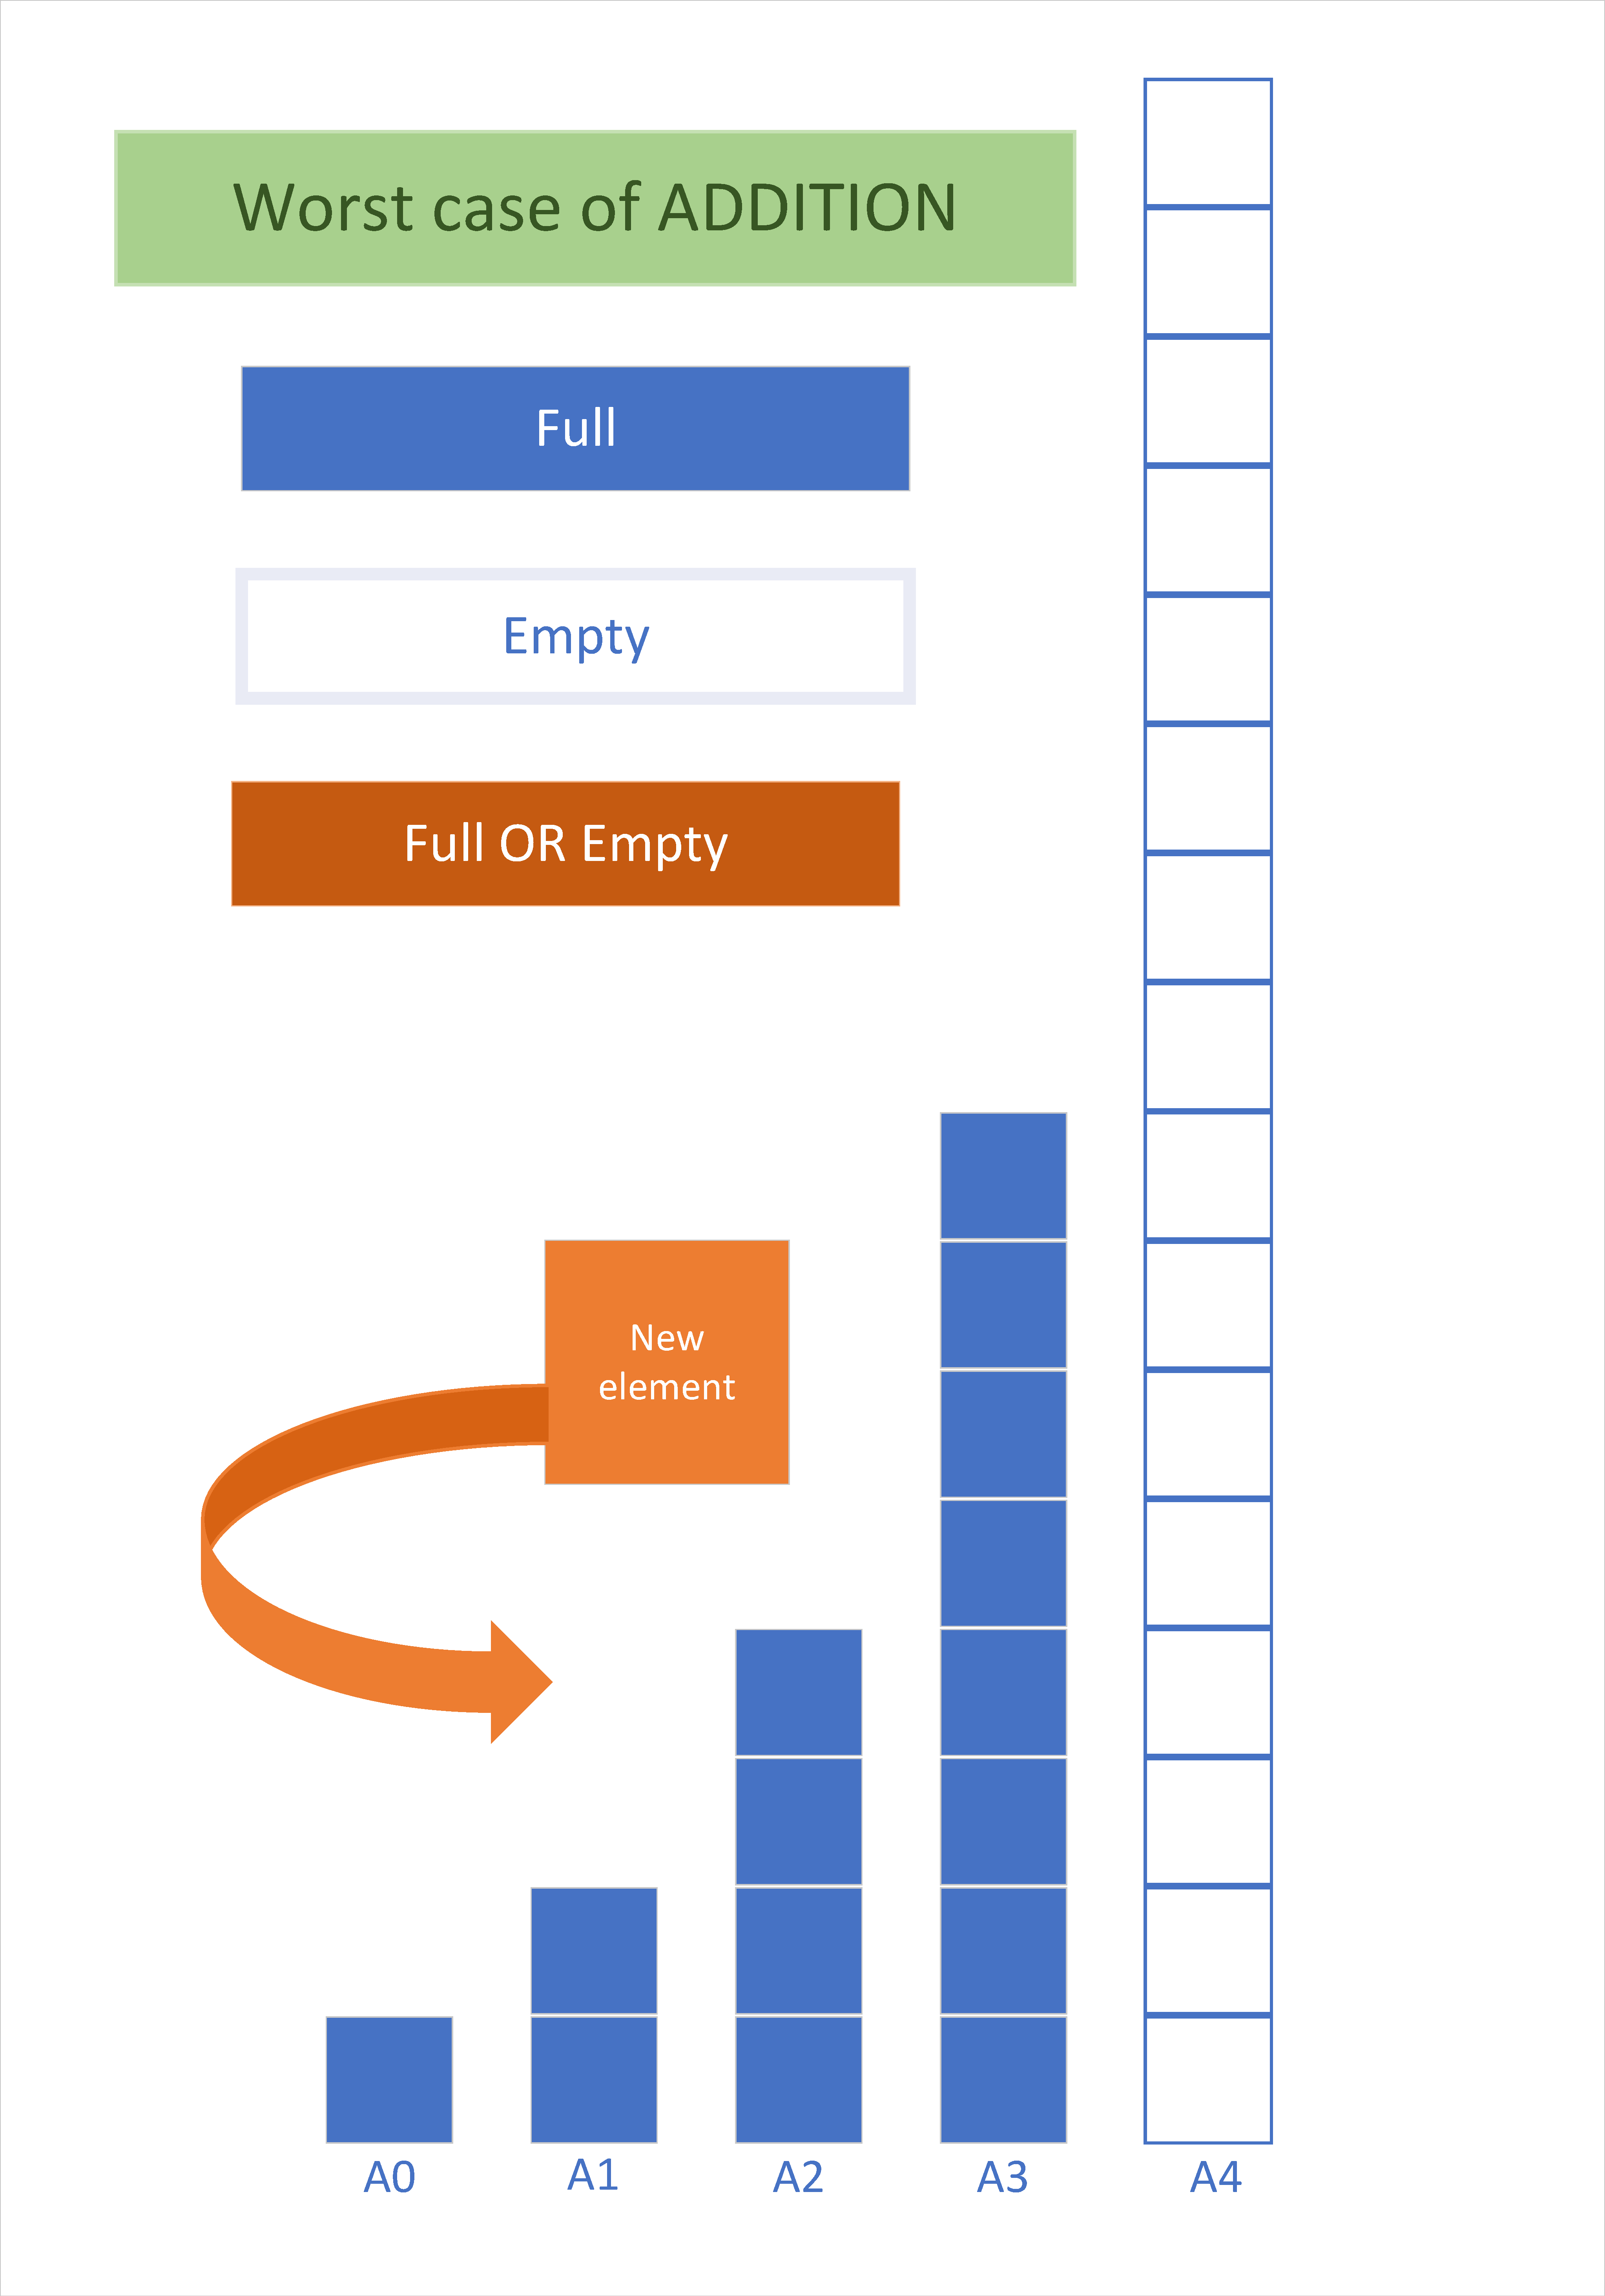
\includegraphics[width=0.4\textwidth]{WorstAddition.pdf}
        	\caption{The worst case of adding an element in the set.}
        	\label{WorstAddition}
    	\end{figure}        
    	
        \item [(b)] 
        \begin{proof}
        ~\\
        Let \textsc{ADDITION} denote the only operation in this question, which adds an element in the set of arrays. 
        \\
        Before calculating the amortized time complexity of the sequence of $n$ operations, let us prove two lemmas.
        \begin{lemma}\label{lemma1}
        Any array in the sets is either empty or full.
        \end{lemma}
        \begin{lemma} \label{lemma2}
        Let $S_i$ represent the state where only $A_i$ is full and $A_0,A_1,\cdots,A_{i-1}$ is empty. In the process of changing $S_0$ to $S_q$ using the \textsc{ADDITION} operation, the array $A_p$ will be filled
        up $2^{q-p-1}$ times.
        \end{lemma}
    
        \textbf{The proof of the two lemmas are shown below the \textit{Amortized time complexity analysis}}.
        \\
    	\begin{figure}[htbp]
        	\centering
        	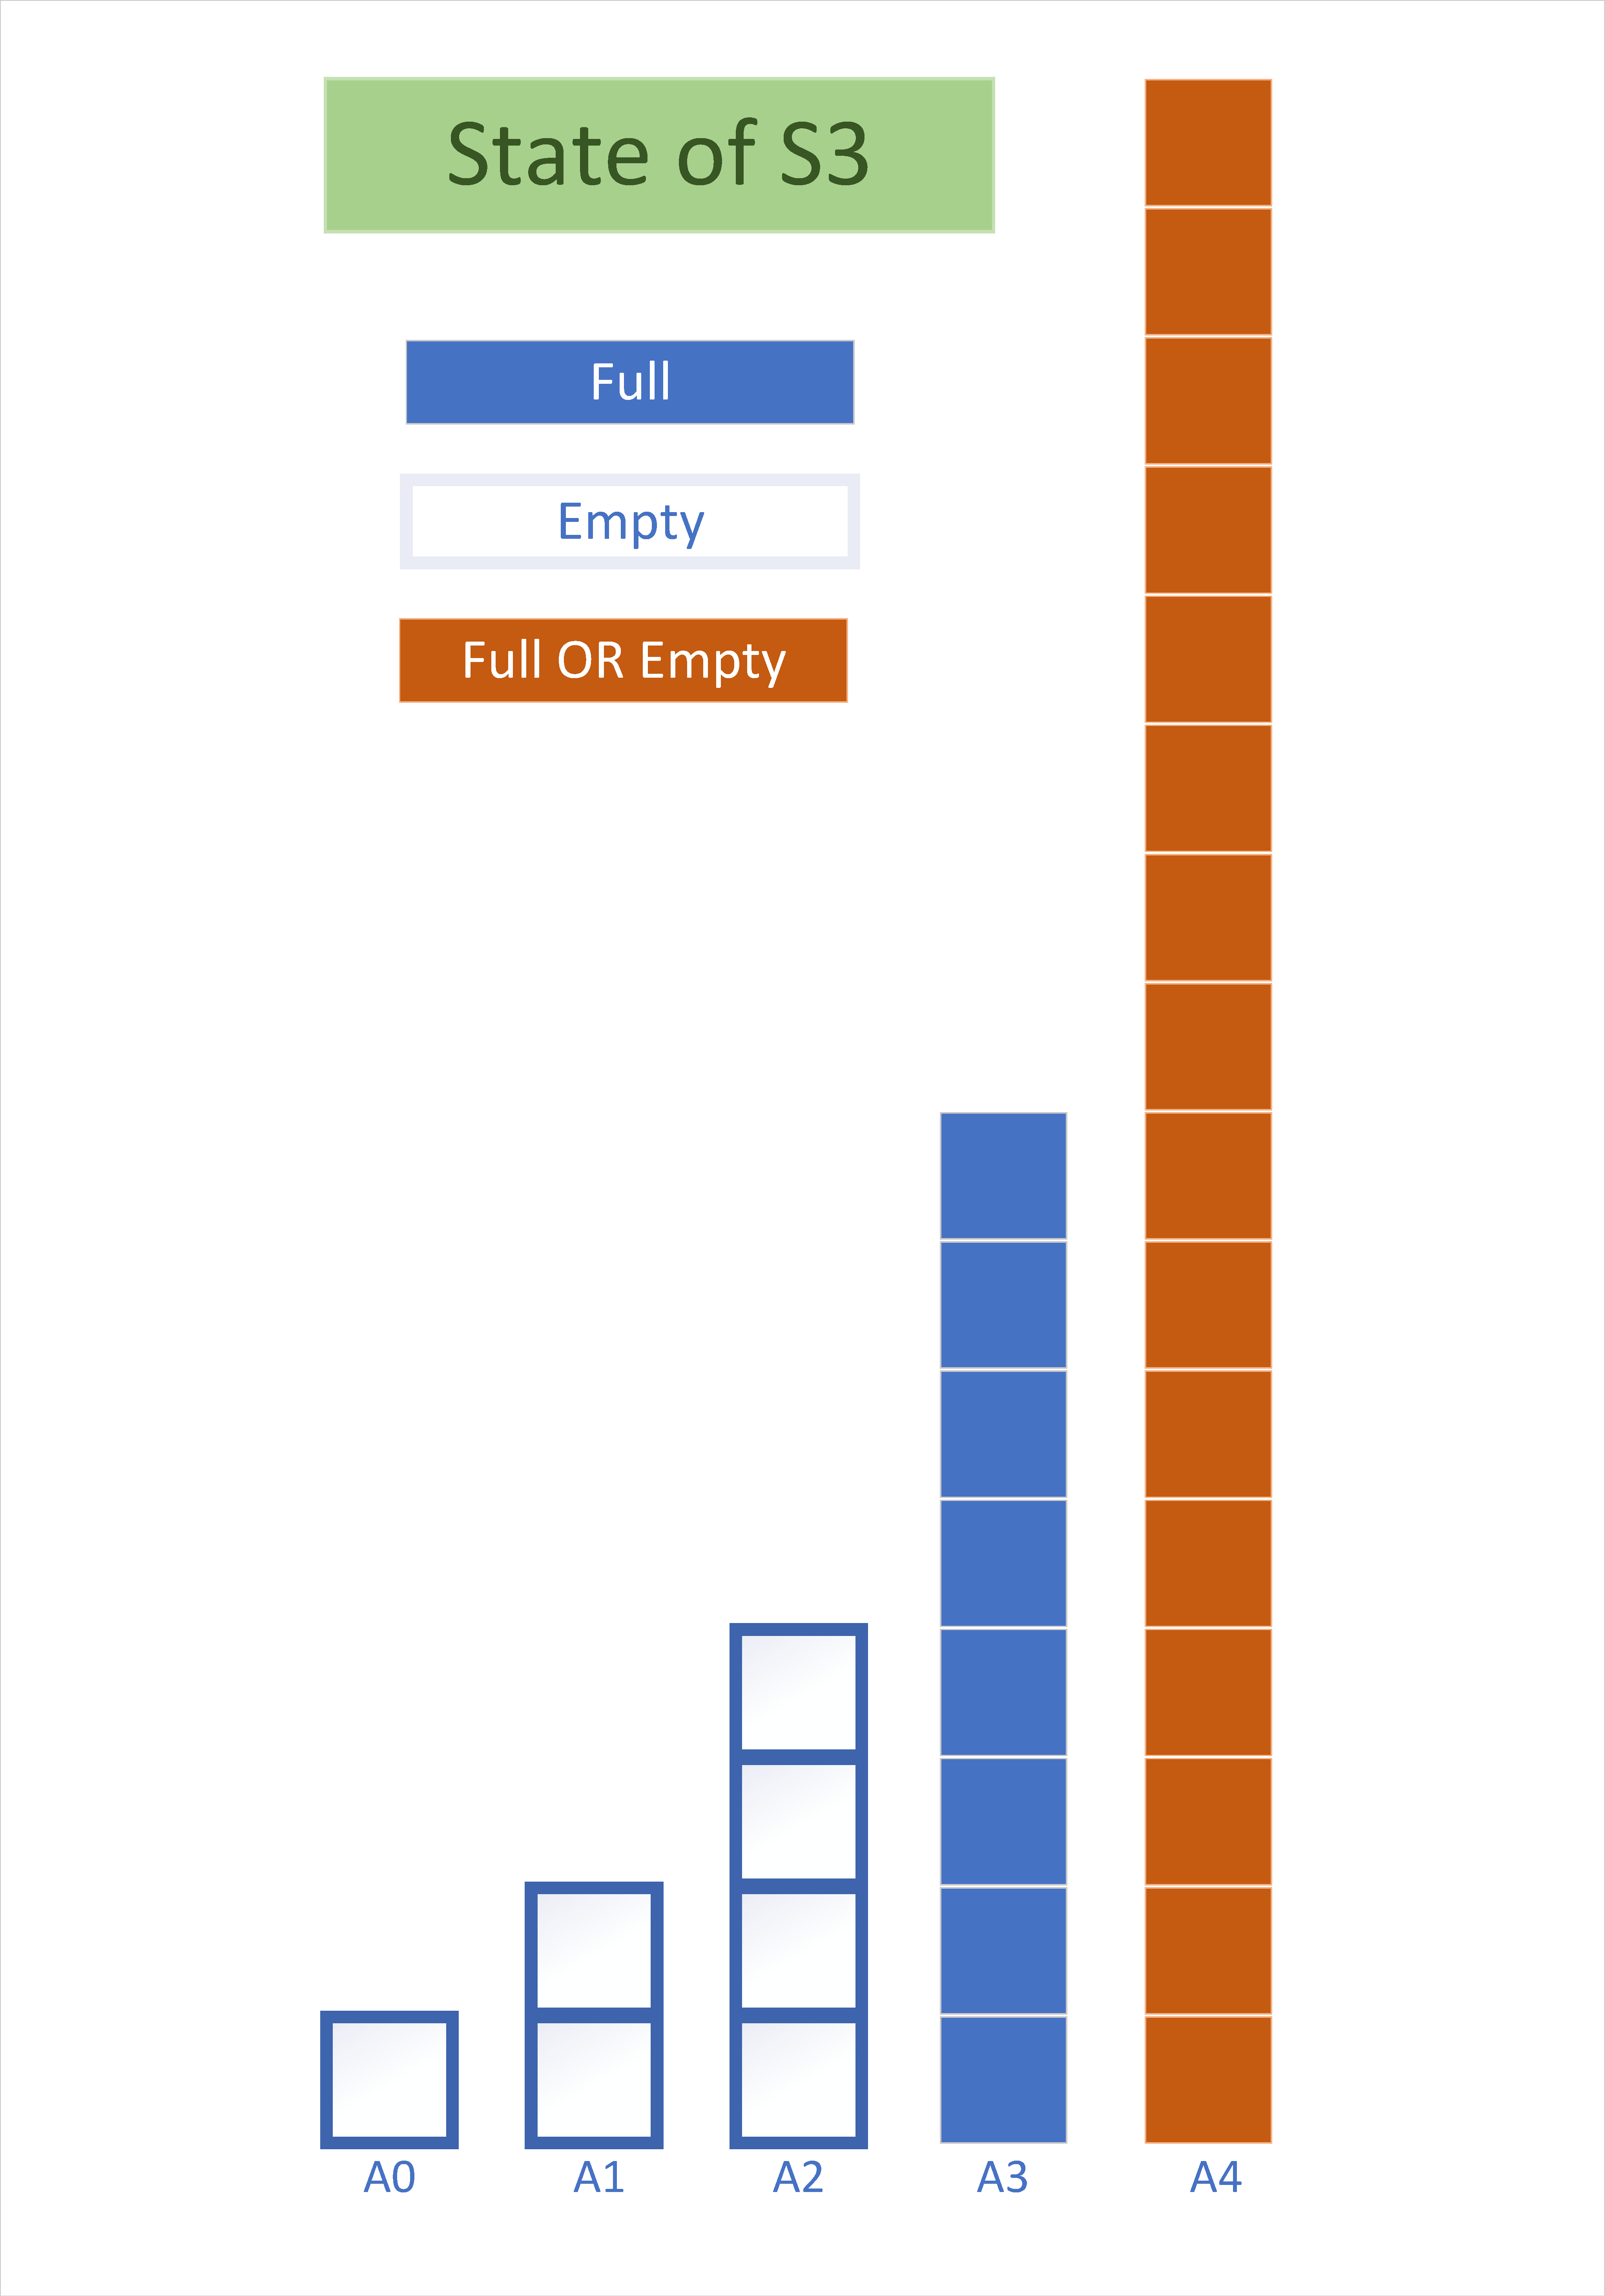
\includegraphics[width=0.4\textwidth]{State.pdf}
        	\caption{Implication of state $S_3$ in Lemma.~\ref{lemma2}}
        	\label{State}
    	\end{figure}   
        ~\\
        \textbf{\textit{Amortized time complexity analysis:}}
        \\
        After $n$ \textsc{ADDITION} operations, the set will contain $n$ elements. Suppose $k$ is the index of the array with the largest index in this set of $n$ elements. We have:
        $$2^k\leq n\leq 1+2^1+2^2+\cdots+2^k=2^{k+1}-1$$
        So
        $$\log (n+1)-1 \leq k\leq \log n$$
        which means
        $$k \sim \Theta(\log n)$$
        Let $\# FILL\ i$ denote the time complexity of changing the set from $S_0$ to $S_i$. 
        
        \begin{equation}
        \begin{split}
            Total\ amortized\ &time\ complexity\\
           & =  \sum_{A_i\ is\ full} \# FILL\ i \\
            & \leq\ \ \  \sum_{i=1}^k\ \ \# FILL\ i \\
            &=\ \ \ \sum_{i=0}^{k-1} 2^{k-i-1} \times (2^i-1) \\
            &=\ \ \ (k-2)2^{k-1}-1\\
            &=\ \ \  (\Theta(\log n) -2)2^{\Theta(\log n)-1}-1\\
            &=\ \ \ \Theta (n\log n)
        \end{split}
        \end{equation}
        And $$\text{Average time complexity}=\frac{O(n\log n)}{n}=O(\log n)$$
        ~\\
        
        
        
        
        \begin{proof} [Proof of Lemma.~\ref{lemma1}] 
        ~\\ 
        ~\\
        \textbf{\textit{Basis step:}} $n=0$: $A_0$ is able to contain only one element, so it is either empty or full. 
        \\
        \textbf{\textit{Induction hypothesis:}} Suppose that for any $n$, where $n\leq k$, $A_n$ is either empty or full.
        \\
        \textbf{\textit{Proof of the induction step:}} Suppose $A_i$ is the first 
        array ahead of $A_{k+1}$ with no element. The number of elements that need to be placed after the \textsc{ADDITION} operation is $(2^0+2^1+\cdots+2^{i-1})+1=2^i$, which is exactly the capacity of $A_i$. As a result, $A_{k+1}$ remains empty after a \textsc{ADDITION} except for $i=k+1$, which means $A_{k+1}$ will be full after the operation.
        \end{proof}   
        ~\\
        \begin{proof} [Proof of Lemma.~\ref{lemma2}]
        ~\\
        ~\\
        Ahead of the operation which changes the state of the set to $S_i$, $A_0,A_1,\cdots,A_{q-1}$ must be full. In addition, the set must have gone through the states of $S_{q-1},S_{q-2},\cdots,S{p}$ in turn. As a result, let $a_{p,q}$ denote the number of $A_p$ being filled from $S_0$ to $S_q$,  we could generate:
        $$a_{p,q}=\sum_{i=p}^{q-1}a_{p,i}$$
        
        Let $q\leftarrow q+1$:
        $$a_{p,q+1}=\sum_{i=p}^{q}a_{p,i}$$
        By subtraction of the two formula we have:
        $$a_{p,q+1}=2a_{p,q}=\cdots=2^{(q+1)-1-p}a_{p,p+1}=2^{(q+1)-1-p}$$
        
        \end{proof}        
        \end{proof}
    \item [(c)]
    The worst case occurs when the $n$ elements occupy $A_0,A_1,\cdots,A_k$ and each element in each array must be detected. The worst case time complexity is 
    \begin{equation}
        \begin{split}
        \text{Time complexity} = &\sum_{i=0}^k O(\log 2^i)\\
            =& O(\log 2^0\times 2^1\times \cdots \times 2^k)\\
            =& O(\log 2^{\frac{(1+k)\times k}{2}})\\
            =& O(\log^2 n)
        \end{split}
    \end{equation}
    since we have proved in (b) that $k\sim O(\log n)$.
    \begin{figure}[htbp]
        	\centering
        	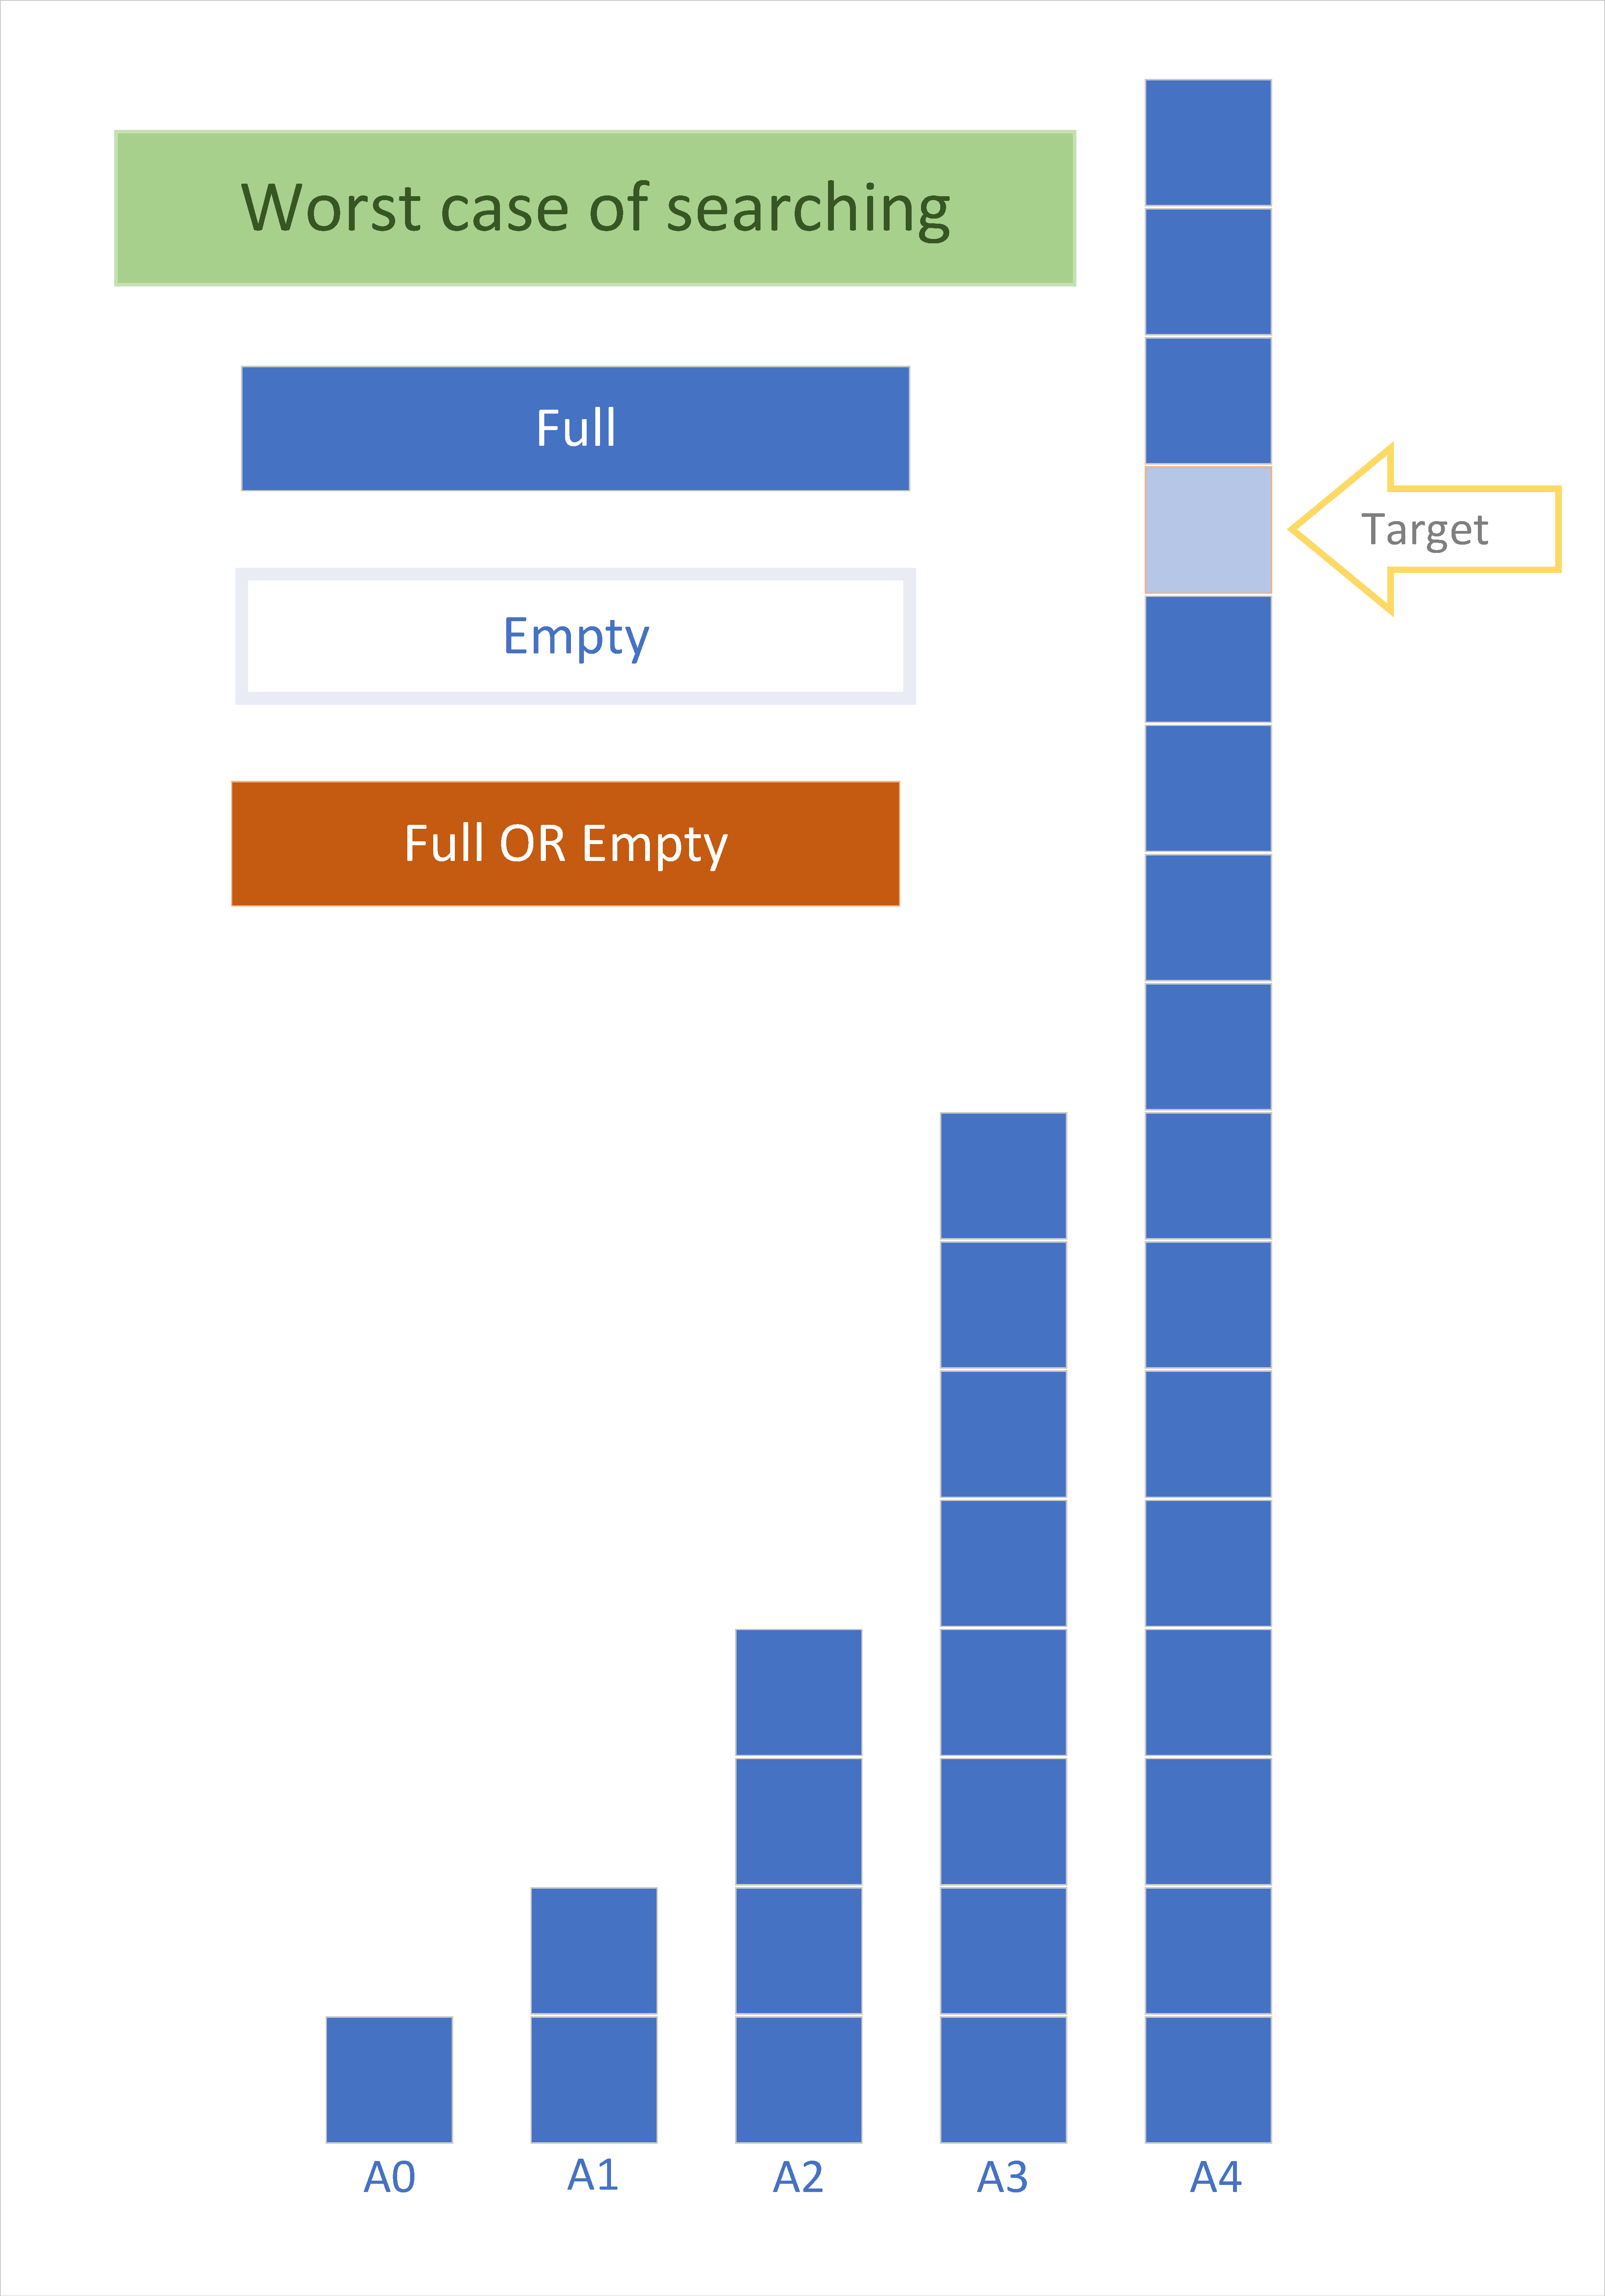
\includegraphics[width=0.4\textwidth]{WorstSearching.pdf}
        	\caption{The worst case of searching an element in the set}
        	\label{WorstSearching}
    	\end{figure}  
    \item[(d)] If $A_0,A_2,\cdots,A_{k-1}$ are full, the time complexity of the operation clearing $A_0,A_2,\cdots,A_{k-1}$ and occupying $A_k$ is
    \begin{equation}\label{Equ-1}
        \begin{split}
            \sum_{i=0}^{k-1} 2^i+O(2^{i+1}-1)
        \end{split}
    \end{equation}
    The former $2^i$ is the time complexity of popping $A_i$. The later $O(2^{i+1}-1)$ is the time complexity of merging sort, which is the fastest method to merge two sorted sequence. 
    \\
    Equation.~\ref{Equ-1} is 
    \begin{equation}
        \begin{split}
            &\sum_{i=0}^{k-1} 2^i+O(2^{i+1}-1)\\
            =& 2^k-1+O(2^k)\\
            =& O(2^k)\\
            =& O(n)
        \end{split}
    \end{equation}
    As a result, the step of merge won't increase time complexity. The amortized time complexity remains 
    $$\text{Amortized time complexity of single operation}= O(\log n)$$ 
    
    \end{enumerate}
    \end{solution}
    \end{enumerate}
	
\end{enumerate}



\textbf{Remark:} Please include your .pdf, .tex files for uploading with standard file names.


%========================================================================
\end{document}
